\section{Analytical expressions for dynamic EM stress of multi-branch}
\label{sec:analytical_expressions}
In this section, we present our analytical solution to the multi-branch interconnect trees. We aimed at the general term of stress evolution. For multi-branch interconnect tree, the stress evolution is still governed by the Korhonen��s equation \eqref{eq:basic_em_s}. In order to analysis the multi-branch interconnect tree, we break it into a number of simple single-segment wires, shown in Fig.\ref{fig:InterconnectTree}. They have different numbers of segments which are connected through the middle node ``0". Each port and branch is identified by number. The current densities in each segment may not be same, which is determined by the rest if the circuit. Then, based on the port 0, we establish rectangular coordinates indicating the location of each branch to induce further solution. The continuity at the joints (port 0) of connected wire segments should be noted.

\begin{figure}[!h]
\centering
\subfigure[]{
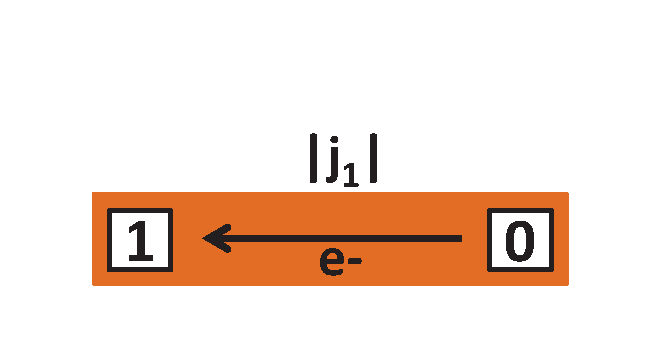
\includegraphics[width=0.45\columnwidth]{tree_1.eps}
\label{fig:singleline}}
\subfigure[]{
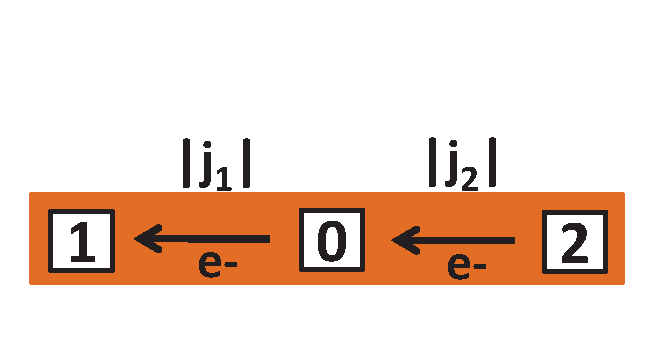
\includegraphics[width=0.45\columnwidth]{tree_2.eps}
\label{fig:straightline}}
\subfigure[]{
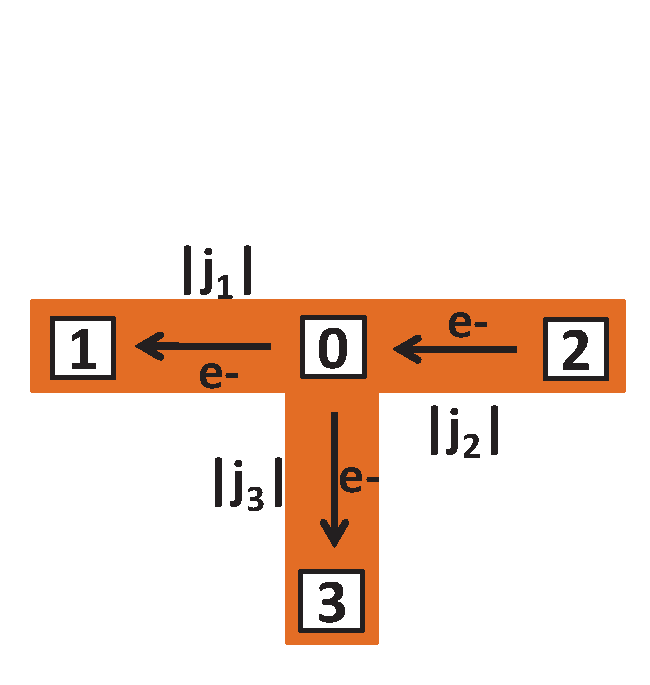
\includegraphics[width=0.45\columnwidth]{tree_3.eps}
\label{fig:Tshaped}}
\subfigure[]{
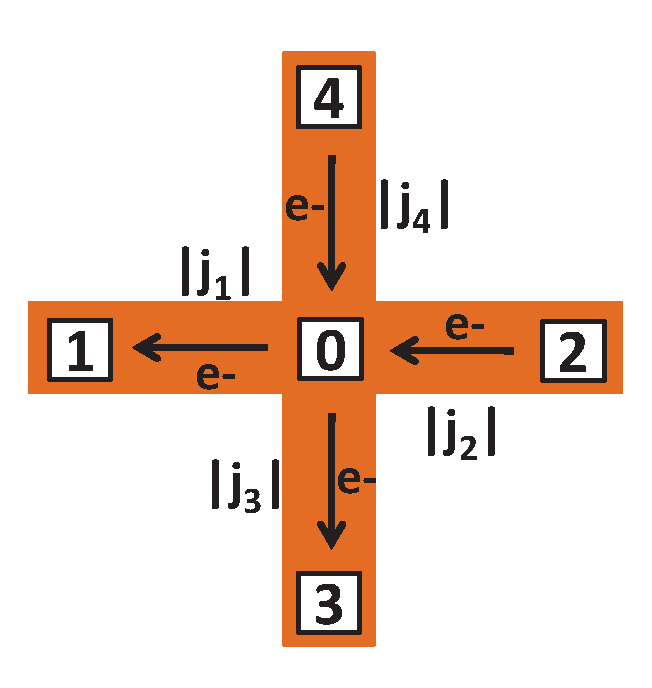
\includegraphics[width=0.45\columnwidth]{tree_4.eps}
\label{fig:Cshaped}}
\caption{Each branch has same length $L$, and the direction of arrow means the direction of current: (a) single line wire; (b) the straight-line there-terminal wires; (c) the T-shaped four-terminal wires; (d) the cross-shaped five-terminal wires.}
\label{fig:InterconnectTree}
\end{figure}

We suppose that the interconnect tree has $k$ branches. Here, the stress model of each segments takes the form in Equations \eqref{eq:tree_basic_em}, in which $m=0,1,...,\lfloor \frac{k}{2}\rfloor$, and $n=0,1,...,\lfloor \frac{k}{2}\rfloor-1$. However, only these equations can not derive the analytical solution of stress evolution.
\begin{equation} \label{eq:tree_basic_em}
\begin{split}
\frac{\partial \sigma_{2m+1}(x,t)}{\partial t}&=\frac{\partial }{\partial
x}[D_{t,2m+1}(\frac{\partial \sigma_{2m+1}(x,t)}{\partial x}+G_{2m+1})]\\
&\qquad\qquad\qquad\qquad\texttt{in}\;-L<x<0,\;t>0,\\
\frac{\partial \sigma_{2n+2}(x,t)}{\partial t}&=\frac{\partial }{\partial
x}[D_{t,2n+2}(\frac{\partial \sigma_{2n+2}(x,t)}{\partial
x}+G_{2n+1})]\\
&\qquad\qquad\qquad\qquad\texttt{in}\;0<x<L,\;t>0.
 \end{split}
 \end{equation}

Furthermore, stresses at the boundary need to be continuous for atom flux being continuous, which is reflected in Boundary Equations \eqref{eq:boundary_equations} (BEs).
\begin{equation} \label{eq:boundary_equations}
\begin{split}
&D_{t,2m+1}(\frac{\partial \sigma_{2m+1}(x,t)}{\partial x}+G_{2m+1})=0,
\texttt{at}\;x=-L,\;t>0,\\
&D_{t,2n+2}(\frac{\partial \sigma_{2n+2}(x,t)}{\partial
x}+G_{2n+2})=0,
\texttt{at}\;x=L,\;t>0,\\
&\sigma_{2m+1}(x,t)=\sigma_{2n+2}(x,t),\;\texttt{at}\;x=0,\;t>0\\
&\sum_{m=0}^{\lfloor \frac{k}{2}\rfloor}D_{t,2m+1}(\frac{\partial \sigma_{2m+1}(x,t)}{\partial
x}+G_{2m+1})\\
&\qquad\qquad\qquad=\sum_{n=0}^{\lfloor \frac{k}{2}\rfloor-1}D_{t,2n+2}(\frac{\partial \sigma_{2n+2}(x,t)}{\partial
x}+G_{2n+2}),\\
&\qquad\qquad\qquad\qquad\qquad\qquad\qquad\qquad\texttt{at}\;x=0,\;t>0
\end{split}
\end{equation}

Meanwhile, there is no stress anywhere in the whole tree at $t = 0$. We definite the Initial Equations (CEs) as follow:
\begin{equation} \label{eq:initial_equations}
\begin{split}
&\sigma(x,t)=0,\;\texttt{at}\;t=0,\;\texttt{for any x}\\
\end{split}
\end{equation}

The Laplace transform of $\sigma(x,t)$ can be defined as $\hat{\sigma}(x,s)=\int_{0}^{+\infty}e^{-st}\sigma(x,t)dt$. Using Laplace transform in Equations \eqref{eq:tree_basic_em} with CEs, we got $\frac{d^2\hat{\sigma}(x,s)}{dx^2}=\frac{s}{D_{t}}\hat{\sigma}(x,s)$, which leads to:
\begin{equation} \label{eq:basic_expression}
\begin{split}
&\hat{\sigma}_{2m+1}(x,s)=A_{2m+1}e^{\sqrt{\frac{s}{D_{t,2m+1}}}x}+B_{2m+1}e^{-\sqrt{\frac{s}{D_{t,2m+1}}}x}\\
&\hat{\sigma}_{2n+2}(x,s)=A_{2n+2}e^{\sqrt{\frac{s}{D_{t,2n+2}}}x}+B_{2n+2}e^{-\sqrt{\frac{s}{D_{t,2n+2}}}x}
\end{split}
\end{equation}

Using Laplace transform and substituting the expressions \eqref{eq:basic_expression} into BEs in turn, we obtained:

\begin{equation}
\begin{split}
&\beta_{2m+1} e^{-\beta_{2m+1} L}A_{2m+1}-\beta_{2m+1} e^{\beta_{2m+1} L}B_{2m+1}=-\frac{G_{2m+1}}{s},\\
&\beta_{2n+2} e^{\beta_{2n+2} L}A_{2n+2}-\beta_{2n+2} e^{-\beta_{2n+2} L}B_{2n+2}=-\frac{G_{2n+2}}{s},\\
&A_{2m+1}+B_{2m+1}-A_{2n+2}-B_{2n+2}=0,\\
&\sum_{m=0}^{\lfloor \frac{k}{2}\rfloor}(D_{t,2m+1}\beta_{2m+1} A_{2m+1}-D_{t,2m+1}\beta_{2m+1} B_{2m+1})\\
&\qquad-\sum_{n=0}^{\lfloor \frac{k}{2}\rfloor-1}(D_{t,2n+2}\beta_{2n+2} A_{2n+2}-D_{t,2n+2}\beta_{2n+2} B_{2n+2})\\
&\qquad=-\sum_{m=0}^{\lfloor \frac{k}{2}\rfloor}D_{t,2m+1}\frac{G_{2m+1}}{s}+\sum_{n=0}^{\lfloor \frac{k}{2}\rfloor-1}D_{t,2n+2}\frac{G_{2n+2}}{s}.
\end{split}
\end{equation}
where $\beta_k=\sqrt{\frac{s}{D_{tk}}},k=1,2,3,4$.

For the sake of simplicity, we assume that each branch has the same diffusivity, i.e. $D_{t1}=D_{t2}=...=D$ and $\beta_1=\beta_2=...=\beta=\sqrt{\frac{s}{D}}$. In order to express the analytical solutions $\sigma_i(x,t)$, we introduce the following functions:
\begin{equation} \label{introNotations}
\begin{split}
&\xi_0(x,q)=4qL-x,\;\;\;\;\;\;\;\;\;\;\eta_0(x,q)=4qL+x,\\
&\xi_1(x,q)=(1+4q)L-x,\;\eta_1(x,q)=(1+4q)L+x,\\
&\xi_2(x,q)=(2+4q)L-x,\;\eta_2(x,q)=(2+4q)L+x,\\
&\xi_3(x,q)=(3+4q)L-x,\;\eta_3(x,q)=(3+4q)L+x,\\
&\xi_4(x,q)=(4+4q)L-x,\;\eta_4(x,q)=(4+4q)L+x,
\end{split}
\end{equation}
where n is a nonnegative integer. Then we construct a basic function:
\begin{equation} \label{basisFunc}
g(x,t)=2\sqrt{\frac{\kappa t}{\pi}}e^{-\frac{x^2}{4\kappa
t}}-x\times\texttt{erfc}\{\frac{x}{2\sqrt{\kappa t}}\}.
\end{equation}
where $\texttt{erfc}\{x\}=\frac{2}{\sqrt{\pi}}\int_x^{+\infty}e^{-t^2}dt$ is the complementary error function. Using the functions mentioned above, we express the exact analytical solutions for the stress evolution in each segment:
\begin{equation} \label{eq:solution_odd}
\begin{split}
\sigma_{2m+1}&(x,t)=\frac{1}{k}\sum\limits_{q=0}^{+\infty}\{2(G_s-G_{2m+1})g(\xi_1,t)+kG_{2m+1}g(\xi_3,t)\\
&-(k-2)G_{2m+1}g(\xi_1,t)-G_s(g(\xi_0,t)+g(\xi_2,t))\}\\
&+\frac{1}{k}\sum\limits_{q=0}^{+\infty}\{2(G_s-G_{2m+1})g(\eta_3,t)+kG_{2m+1}g(\eta_1,t)\\
&-(k-2)G_{2m+1}g(\eta_3,t)-G_s(g(\eta_2,t)+g(\eta_4,t))\},\\
 \end{split}
 \end{equation}
\begin{equation} \label{eq:solution_even}
\begin{split}
\sigma_{2n+2}&(x,t)=\frac{1}{k}\sum\limits_{q=0}^{+\infty}\{2(G_s+G_{2n+2})g(\xi_3,t)-kG_{2n+2}g(\xi_1,t)\\
&+(k-2)G_{2n+2}g(\xi_3,t)-G_s(g(\xi_2,t)+g(\xi_4,t))\}\\
&+\frac{1}{k}\sum\limits_{q=0}^{+\infty}\{2(G_s+G_{2n+2})g(\eta_1,t)-kG_{2n+2}g(\eta_3,t)\\
&+(k-2)G_{2n+2}g(\eta_1,t)-G_s(g(\eta_0,t)+g(\eta_2,t))\}.
 \end{split}
 \end{equation}
where $G_s=\sum_{i=0}^{\lfloor\frac{k}{2}\rfloor}G_{2i+1}-\sum_{j=0}^{\lfloor\frac{k}{2}\rfloor-1}G_{2j+2}$
